\section{Neural Network-based Model}
Hệ thống bắt đầu bằng việc tiếp nhận tập hợp các tài liệu văn bản đầu vào, chẳng hạn như các bài báo, mô tả sản phẩm hoặc đoạn văn bản trong một cơ sở dữ liệu lớn. Các tài liệu này sẽ được chuẩn bị để đưa vào mô hình học sâu, thường là một mô hình như BERT (Bidirectional Encoder Representations from Transformers) hoặc một mô hình tương tự.

Thay vì chỉ thực hiện các bước tiền xử lý đơn giản như trong VSM và các bước đó có thể ảnh hưởng đến ngữ nghĩa của toàn câu nên văn bản ở đây sẽ được mã hóa bằng tokenizer chuyên dụng của mô hình BERT, tạo ra chuỗi token được ánh xạ sang các chỉ số từ vựng đã được huấn luyện trước. Sau đó, mô hình BERT xử lý văn bản để tạo ra biểu diễn ngữ nghĩa dưới dạng vector -- còn gọi là document embedding vector. Vector này là một biểu diễn dày đặc (dense representation), mang thông tin ngữ cảnh sâu và mối liên kết giữa các từ trong tài liệu.

Các vector biểu diễn tài liệu này được lưu trữ và lập chỉ mục trong một hệ thống tìm kiếm dựa trên vector như FAISS hoặc Annoy. Việc lập chỉ mục vector cho phép thực hiện truy vấn gần đúng (approximate nearest neighbor search), giúp tăng tốc đáng kể quá trình truy vấn trong không gian nhiều chiều.

Tương tự như tài liệu, truy vấn từ người dùng cũng được đưa qua tokenizer và mô hình BERT để mã hóa thành một vector embedding. Truy vấn có thể là một câu hỏi ngắn hoặc một cụm từ tìm kiếm, và được xử lý theo cùng pipeline như văn bản.

Khi vector embedding của truy vấn đã được tạo, hệ thống sử dụng chỉ mục vector đã lập từ trước để tìm ra các vector tài liệu gần nhất với vector truy vấn -- thường được đo bằng độ tương đồng cosine hoặc tích vô hướng. Các tài liệu có vector càng gần với vector truy vấn được xem là càng phù hợp.

Cuối cùng, hệ thống xếp hạng các tài liệu theo mức độ tương đồng với truy vấn và trả về danh sách các tài liệu liên quan nhất. Đây chính là đầu ra của hệ thống -- danh sách kết quả truy xuất được sắp xếp theo độ liên quan cao đến thấp, mang lại trải nghiệm tìm kiếm hiệu quả và thông minh hơn so với các phương pháp dựa trên thống kê truyền thống.

\begin{figure}[H]
    \caption{Sơ đồ hệ thống của Neural Network-based Model}
    \begin{center}
        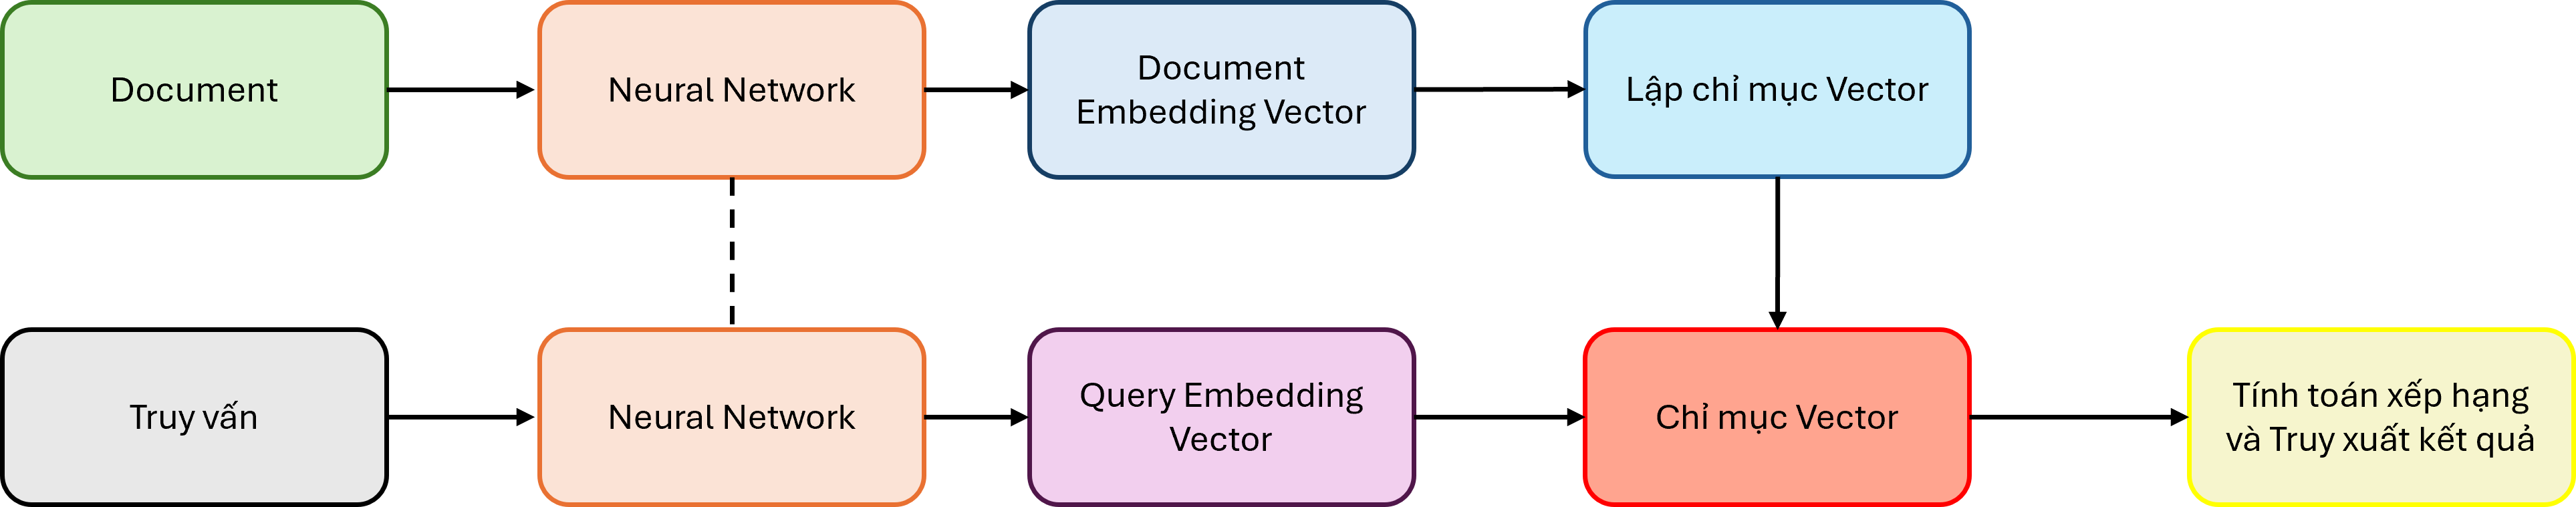
\includegraphics[width=\linewidth]{assets/nn-based-flowchart.png}
    \end{center}
\end{figure}

Nhóm cũng thực hiện thực nghiệm trên tập dữ liệu Cranfield bằng cách sử dụng mô hình Neural Network để cải thiện chất lượng truy xuất. Cụ thể, nhóm sử dụng mô hình \texttt{sentence-transformers/all-MiniLM-L6-v2} để biểu diễn các câu truy vấn và văn bản tài liệu dưới dạng vector embedding. Đây là một mô hình được huấn luyện dựa trên kiến trúc \textbf{MiniLM}, tối ưu hóa cho bài toán \textit{semantic textual similarity}, đặc biệt hiệu quả trong các tác vụ truy hồi văn bản nhờ vào khả năng học được biểu diễn ngữ nghĩa giàu thông tin ở dạng vector chiều thấp.

\textbf{Mô hình \texttt{all-MiniLM-L6-v2}} là một trong những phiên bản nhẹ và nhanh của họ mô hình MiniLM. Mặc dù chỉ sử dụng 6 tầng Transformer (so với 12 tầng trong \texttt{all-MiniLM-L12-v2}), mô hình này được huấn luyện bằng kỹ thuật distillation từ các mô hình lớn hơn, giúp duy trì hiệu suất cao trong khi giảm đáng kể thời gian tính toán và bộ nhớ. Trên thực tế, nhiều đánh giá cho thấy \texttt{MiniLM-L6-v2} đạt chất lượng tương đương hoặc thậm chí tốt hơn \texttt{MiniLM-L12-v2} trong các tác vụ truy hồi, nhờ việc cân bằng tốt giữa độ sâu mô hình và khả năng tổng quát hóa. Ngoài ra, do mô hình nhẹ hơn, embedding sinh ra từ \texttt{MiniLM-L6-v2} có xu hướng ít nhiễu và ổn định hơn đối với tập dữ liệu nhỏ như Cranfield.

Sau khi biểu diễn các tài liệu và truy vấn dưới dạng vector, nhóm sử dụng thư viện \textbf{FAISS (Facebook AI Similarity Search)} để xây dựng chỉ mục truy xuất nhanh. FAISS là một thư viện tối ưu cao được phát triển bởi Facebook AI Research, chuyên dùng để tìm kiếm gần đúng các vector trong không gian chiều cao (Approximate Nearest Neighbor Search). FAISS hỗ trợ nhiều cấu trúc dữ liệu như flat index, HNSW, IVF để đảm bảo cân bằng giữa tốc độ truy vấn và độ chính xác.

Trong thử nghiệm này, nhóm sử dụng FAISS để lập chỉ mục các vector văn bản và thực hiện truy vấn bằng cách tìm kiếm \(k\) vector gần nhất (top-\(k\)) với vector truy vấn trong không gian embedding. Vì tập Cranfield có kích thước nhỏ (1400 tài liệu), nên nhóm sử dụng \texttt{IndexFlatIP} (Inner Product) --- một phương pháp đơn giản nhưng hiệu quả trong không gian embedding được chuẩn hóa.

Cách tiếp cận này giúp hệ thống truy xuất không còn phụ thuộc vào từ khóa trực tiếp mà thay vào đó tận dụng mối quan hệ ngữ nghĩa giữa các câu, dẫn đến kết quả truy vấn chính xác hơn trong nhiều trường hợp, đặc biệt là với các truy vấn ngắn hoặc có ngữ nghĩa rộng.

Sau khi xây dựng hệ thống truy xuất dựa trên mô hình embedding ngữ nghĩa kết hợp với FAISS index, nhóm tiến hành đánh giá chất lượng truy xuất bằng cùng bộ truy vấn như đối với mô hình VSM. Các chỉ số đo lường được báo cáo như sau:

\begin{itemize}
    \item \textbf{Mean Precision@10}: 0.2489
    \item \textbf{Mean Recall@10}: 0.4177
    \item \textbf{Mean Average Precision (MAP)}: 0.3264
\end{itemize}

Các chỉ số trên cho thấy mô hình học sâu kết hợp với biểu diễn embedding ngữ nghĩa đã đạt được kết quả tốt hơn so với mô hình VSM truyền thống. Giá trị Precision@10 và Recall@10 đều tăng lên, cho thấy khả năng truy xuất chính xác và bao phủ cao hơn ở top kết quả đầu tiên. Đặc biệt, chỉ số MAP tăng rõ rệt, phản ánh sự cải thiện tổng thể trong chất lượng truy xuất.
